%!TeX root=../main.tex

\chapter{Distribuzione e prodotto finale}\label{ch:distribuzione-e-prodotto-finale}

\section{Strategia di distribuzione}\label{sec:strategia-di-distribuzione}
La fase di distribuzione ha avuto come obiettivo non solo il rilascio tecnico dell’applicazione, ma anche la validazione della sua utilizzabilità in un ambiente che simula condizioni reali di produzione.
Per \textbf{Swift Contest} è stato scelto un approccio multipiattaforma che copre i principali punti di accesso per i diversi tipi di utenti:
\begin{itemize}
    \item \textbf{Applicazione Web}: distribuita su \textbf{Vercel}, per garantire accessibilità universale da qualsiasi browser moderno, sia desktop che mobile.
    \item \textbf{Applicazione Android}: distribuita come pacchetto APK, reso disponibile tramite un meccanismo di download sicuro per un'esperienza d'uso ottimizzata su dispositivi mobili.
    \item \textbf{Infrastruttura Backend}: interamente gestita su \textbf{Supabase}, che ospita il database, lo storage, le funzioni serverless e i servizi realtime.
    \item \textbf{Pannello di Amministrazione}: sviluppato come strumento interno su \textbf{Retool} e interfacciato in modo sicuro con il backend, per le attività di moderazione e manutenzione.
\end{itemize}
Questa strategia ibrida consente di bilanciare la facilità di accesso (garantita dalla versione Web) con un'esperienza d'uso ottimizzata (offerta dalla versione Android), mantenendo al contempo un backend centralizzato, sicuro e scalabile.

\begin{figure}[H]
    \centering
    
\includegraphics[width=\textwidth]{capitoli/figure/diagrams/deployment-diagram}
    \caption{Diagramma di distribuzione dell'architettura completa di Swift Contest.}
    \label{fig:deployment_diagram}
\end{figure}

\section{Distribuzione web su Vercel}\label{sec:distribuzione-web-su-vercel}
La versione Web dell'applicazione Flutter è stata distribuita su Vercel~\cite{vercel_website}, una piattaforma serverless ottimizzata per la distribuzione di frontend moderni.
Il processo è completamente automatizzato tramite una pipeline di \textbf{CI/CD (Continuous Integration/Continuous Deployment)} integrata con il repository Git del progetto.
Ogni \emph{push} sul branch \texttt{main} innesca automaticamente una nuova build dell'applicazione Flutter in modalità \emph{release} e una conseguente distribuzione sulla piattaforma.

Per garantire il corretto funzionamento di una \emph{Single Page Application (SPA)} come Flutter Web, è stato configurato un file \texttt{vercel.json} che gestisce il rewrite di tutte le rotte verso il file \texttt{index.html}, permettendo al router di Flutter (\texttt{auto\_route}) di gestire la navigazione lato client.

\section{Distribuzione Android}\label{sec:distribuzione-android}
Per la piattaforma Android, è stata prodotta una \textbf{release in formato APK}.
Data la natura prototipale del progetto, si è evitato il complesso processo di pubblicazione sul Google Play Store, optando per un approccio di distribuzione controllata che garantisce comunque sicurezza e facilità di aggiornamento:
\begin{enumerate}
    \item L'APK viene caricato come \emph{release asset} (un file allegato a una specifica versione del software) su un repository GitHub~\cite{github_website} privato.
    \item Un'apposita Edge Function, \texttt{get-latest-apk}, è stata creata su Supabase per fungere da proxy sicuro.
    Questa funzione utilizza un \textbf{Personal Access Token (PAT)} di GitHub, memorizzato in modo sicuro in Supabase, per autenticarsi all'API di GitHub e scaricare l'asset.
    \item L'applicazione web offre un pulsante ``Download for Android'' che invoca questa Edge Function.
    L'utente riceve così l'ultima versione dell'APK direttamente dal backend, senza che il repository GitHub o le credenziali di accesso vengano mai esposte.
\end{enumerate}

\begin{figure}[H]
    \centering
    
\includegraphics[width=0.30\textwidth]{capitoli/figure/web/sign-up}
    \caption{Pagina di accesso dell'applicazione web distribuita su Vercel.}
    \label{fig:web-sign-up}
\end{figure}

\section{Backend e Supabase}\label{sec:backend-e-supabase}
L'intera infrastruttura backend è gestita su Supabase.
Il processo di distribuzione del database è basato su migrazioni SQL, seguendo le pratiche di \textbf{Infrastructure as Code (IaC)}.
Ogni modifica allo schema del database, alle policy RLS o alle funzioni RPC è definita in un file \texttt{.sql} all'interno della cartella \texttt{supabase/migrations}.
La CLI di Supabase viene utilizzata per applicare queste migrazioni in modo sequenziale e versionato, garantendo che l'ambiente di produzione sia sempre allineato con la definizione del codice.
Le Edge Functions, scritte in TypeScript, vengono anch'esse distribuite tramite la CLI\@.

\begin{longtable}{p{0.20\textwidth} p{0.40\textwidth} p{0.30\textwidth}}
    \toprule
    \textbf{Componente} & \textbf{Utilizzo nel Progetto Swift Contest} & \textbf{Implementazione / Note Tecniche} \\
    \midrule
    \endfirsthead
    \toprule
    \textbf{Componente} & \textbf{Utilizzo nel Progetto Swift Contest} & \textbf{Implementazione / Note Tecniche} \\
    \midrule
    \endhead

    \textbf{Database} \newline (PostgreSQL) &
    Persistenza di tutti i dati applicativi: utenti, contest, partecipazioni, giurie, voti, ecc.
    È il ``single source of truth'' del sistema.
    &
    Schema e logica definiti tramite file di migrazione SQL nella cartella \texttt{supabase/migrations}. \\
    \midrule

    \textbf{Auth} &
    Gestione completa del ciclo di vita degli utenti: registrazione, login, autenticazione anonima e gestione delle sessioni tramite JWT. &
    Integrato tramite la libreria \texttt{supabase-flutter}.
    La tabella \texttt{auth.users} è estesa dalla tabella \texttt{public.profiles}. \\
    \midrule

    \textbf{Storage} &
    Archiviazione sicura di tutti i file binari caricati dagli utenti, come le immagini dei contest e i file dei lavori.
    &
    Nessun file è pubblico.
    L'accesso avviene esclusivamente tramite \emph{signed URL} temporanei generati lato server. \\
    \midrule

    \textbf{Edge Functions} &
    Esecuzione di logica server-side complessa, orchestrazione di operazioni multi-servizio e interazione con API esterne.
    &
    Scritte in TypeScript (runtime Deno) e distribuite dalla cartella \texttt{supabase/functions}. \\
    \midrule

    \textbf{Funzioni RPC} &
    Punto di ingresso primario per la logica di business confinata al database.
    &
    Scritte in PL/pgSQL e definite nei file di migrazione. \\
    \midrule

    \textbf{Realtime} &
    Propagazione di modifiche del database ai client sottoscritti in tempo reale per notifiche e aggiornamenti di stato.
    &
    L'autorizzazione alla sottoscrizione è gestita tramite policy RLS di tipo \texttt{SELECT}. \\

    \bottomrule
    \caption{Riepilogo delle componenti Supabase e del loro utilizzo nel progetto.}
    \label{tab:supabase_components}
\end{longtable}

\section{Dashboard amministrativa (Retool)}\label{sec:dashboard-amministrativa-(retool)}
Per le attività di amministrazione avanzata, come la moderazione degli utenti e la gestione dei contenuti, è stata creata una dashboard interna utilizzando \textbf{Retool}~\cite{retool_website}.
Questa interfaccia, non esposta agli utenti finali, comunica con il backend Supabase attraverso un'API sicura, come descritto nel capitolo precedente.

\begin{figure}[H]
    \centering
    
\includegraphics[width=0.6\textwidth]{capitoli/figure/admin/retool-dashboard}
    \caption{La dashboard di amministrazione sviluppata in Retool, che mostra l'elenco degli utenti registrati.}
    \label{fig:retool-dashboard}
\end{figure}

\section{Prodotto finale: interfaccia utente e flussi operativi}\label{sec:prodotto-finale}
In questa sezione viene presentato il prodotto finale attraverso un'analisi visuale dei suoi \textbf{flussi operativi principali}.
L'obiettivo non è quello di documentare ogni singola schermata dell'applicazione, ma di illustrare, tramite l'interfaccia utente (UI), i percorsi più significativi per ciascuno degli attori del sistema.

Partendo dalle schermate di base, come l'autenticazione e le impostazioni, verranno poi illustrati i flussi specifici per l'\textbf{Organizzatore}, il \textbf{Partecipante}, il \textbf{Giurato Nominato} e il \textbf{Giurato Semplice} (ospite).

\subsection{Accesso e autenticazione}\label{subsec:accesso-e-autenticazione}
L'accesso all'applicazione inizia con una \textbf{Splash Screen} che gestisce l'inizializzazione dei servizi principali.
Successivamente, l'utente viene indirizzato al flusso di autenticazione, che comprende le pagine di \textbf{Sign In} (per l'accesso) e \textbf{Sign Up} (per la registrazione di un nuovo account).

\begin{figure}[H]
    \centering
    \begin{minipage}[t]{0.30\textwidth}
        \centering
        
\includegraphics[width=\linewidth]{capitoli/figure/splash}
        \subcaption{Splash screen}
        \label{fig:splash}
    \end{minipage}\hfill
    \begin{minipage}[t]{0.30\textwidth}
        \centering
        
\includegraphics[width=\linewidth]{capitoli/figure/auth/sign-in}
        \subcaption{Pagina di sign in}
        \label{fig:signin}
    \end{minipage}\hfill
    \begin{minipage}[t]{0.30\textwidth}
        \centering
        
\includegraphics[width=\linewidth]{capitoli/figure/auth/sign-up}
        \subcaption{Pagina di sign up}
        \label{fig:signup}
    \end{minipage}
    \caption{Le schermate del flusso di autenticazione dell'applicazione.}
    \label{fig:auth-flow}
\end{figure}

\subsection{Gestione delle impostazioni}\label{subsec:gestione-impostazioni}
Una volta autenticato, ogni utente ha accesso a una sezione dedicata alle impostazioni.
La pagina delle \textbf{Impostazioni Generali} offre diverse funzionalità:
\begin{itemize}
    \item Permette di cambiare il \textbf{tema} dell'applicazione (chiaro, scuro o di sistema).
    \item Consente di impostare il \textbf{ruolo preferito} (es. Organizzatore, Partecipante), che determina quale dashboard verrà mostrata all'avvio dell'app.
    \item Fornisce l'accesso ai documenti legali, come i \textbf{Termini di Servizio} e l'\textbf{Informativa sulla Privacy}.
    \item Contiene il pulsante per effettuare il \textbf{logout}.
\end{itemize}
Da qui, l'utente può inoltre navigare alla pagina \textbf{Impostazioni Account}, dove può modificare i dati del proprio profilo o procedere con l'eliminazione sicura del proprio account.

\begin{figure}[H]
    \centering
    \begin{minipage}[t]{0.30\textwidth}
        \centering
        
\includegraphics[width=\linewidth]{capitoli/figure/settings}
        \subcaption{Pagina delle impostazioni generali}
        \label{fig:settings}
    \end{minipage}
    \quad
    \begin{minipage}[t]{0.30\textwidth}
        \centering
        
\includegraphics[width=\linewidth]{capitoli/figure/account-settings}
        \subcaption{Pagina impostazioni account}
        \label{fig:account_settings}
    \end{minipage}
    \caption{Le schermate per la gestione delle impostazioni dell'app e dell'account utente.}
    \label{fig:settings-flow}
\end{figure}

\subsection{Flusso dell'organizzatore}\label{subsec:flusso-organizzatore}
L'organizzatore è l'attore con il set di funzionalità più ricco.
Il suo percorso inizia dalla \textbf{Home Page}, che funge da dashboard principale, mostrando l'elenco dei contest da lui creati.

\begin{figure}[H]
    \centering
    
\includegraphics[width=0.30\textwidth]{capitoli/figure/organizer/home}
    \caption{La home page dell'organizzatore.}
    \label{fig:organizer_home}
\end{figure}

\paragraph{Creazione di un nuovo contest}
Dalla home page, l'organizzatore può avviare la creazione di un nuovo contest tramite un \textbf{form multi-step} che semplifica l'inserimento delle informazioni, suddivise in tre passaggi logici:
\begin{enumerate}
    \item \textbf{Dati Principali}: nome, descrizione, data e luogo del contest.
    \item \textbf{Immagini}: caricamento delle immagini di copertina.
    \item \textbf{Periodo di Sottomissione}: definizione delle date di inizio e fine per la sottomissione dei lavori.
\end{enumerate}

\begin{figure}[H]
    \centering
    \begin{minipage}[t]{0.30\textwidth}
        \centering
        
\includegraphics[width=\linewidth]{capitoli/figure/organizer/create-contest-step1}
        \subcaption{Passo 1: dati principali}
        \label{fig:create_contest_1}
    \end{minipage}\hfill
    \begin{minipage}[t]{0.30\textwidth}
        \centering
        
\includegraphics[width=\linewidth]{capitoli/figure/organizer/create-contest-step2}
        \subcaption{Passo 2: immagini}
        \label{fig:create_contest_2}
    \end{minipage}\hfill
    \begin{minipage}[t]{0.30\textwidth}
        \centering
        
\includegraphics[width=\linewidth]{capitoli/figure/organizer/create-contest-step3}
        \subcaption{Passo 3: periodo sottomissione}
        \label{fig:create_contest_3}
    \end{minipage}
    \caption{Le tre schermate del form guidato per la creazione di un nuovo contest.}
    \label{fig:create_contest_flow}
\end{figure}

\paragraph{Configurazione dei dettagli del contest}
Selezionando un contest, l'organizzatore accede al pannello di gestione, organizzato in tab, da cui può configurare ogni aspetto:
\begin{itemize}
    \item La tab \textbf{Details} mostra un riepilogo delle informazioni generali.
    \item La tab \textbf{Participants} permette di gestire e invitare i partecipanti.
    \item La tab \textbf{Juries} consente di creare e gestire le giurie.
    \item La tab \textbf{Works} mostra l'elenco dei lavori sottomessi.
\end{itemize}

\begin{figure}[H]
    \centering
    \begin{minipage}[t]{0.30\textwidth}
        \centering
        
\includegraphics[width=\linewidth]{capitoli/figure/organizer/contest-details}
        \subcaption{Tab ``Details''}
        \label{fig:contest_details}
    \end{minipage}
    \quad
    \begin{minipage}[t]{0.30\textwidth}
        \centering
        
\includegraphics[width=\linewidth]{capitoli/figure/organizer/contest-participants}
        \subcaption{Tab ``Participants''}
        \label{fig:contest_participants}
    \end{minipage}
    \vspace{1em}
    \begin{minipage}[t]{0.30\textwidth}
        \centering
        
\includegraphics[width=\linewidth]{capitoli/figure/organizer/contest-juries}
        \subcaption{Tab ``Juries''}
        \label{fig:contest_juries}
    \end{minipage}
    \quad
    \begin{minipage}[t]{0.30\textwidth}
        \centering
        
\includegraphics[width=\linewidth]{capitoli/figure/organizer/contest-works}
        \subcaption{Tab ``Works''}
        \label{fig:contest_works}
    \end{minipage}
    \caption{Le principali tab di gestione all'interno di un contest.}
    \label{fig:contest_management_tabs}
\end{figure}

In particolare, la gestione delle giurie prevede una schermata di dettaglio il cui contenuto \textbf{varia a seconda del tipo di giuria}:
\begin{itemize}
    \item Per una \textbf{giuria nominata (\emph{appointed})}, la pagina mostra l'elenco dei giurati.
    \item Per una \textbf{giuria semplice (\emph{simple})}, la pagina espone il \textbf{token} di accesso.
\end{itemize}
Per entrambe, è possibile accedere alla configurazione del \textbf{Voting Form} associato.

\begin{figure}[H]
    \centering
    \begin{minipage}[t]{0.30\textwidth}
        \centering
        
\includegraphics[width=\linewidth]{capitoli/figure/organizer/appointed-jury}
        \subcaption{Dettagli giuria nominata}
        \label{fig:jury_details_appointed}
    \end{minipage}\hfill
    \begin{minipage}[t]{0.30\textwidth}
        \centering
        
\includegraphics[width=\linewidth]{capitoli/figure/organizer/jury-voting-form}
        \subcaption{Configurazione voting form}
        \label{fig:voting_form_edit}
    \end{minipage}\hfill
    \begin{minipage}[t]{0.30\textwidth}
        \centering
        
\includegraphics[width=\linewidth]{capitoli/figure/organizer/simple-jury}
        \subcaption{Dettagli giuria semplice}
        \label{fig:jury_details_simple}
    \end{minipage}
    \caption{Le viste di dettaglio per i due tipi di giuria e la configurazione del Voting Form.}
    \label{fig:jury_and_form_views}
\end{figure}

\paragraph{Gestione della sessione di voto}
La tab \textbf{Voting} permette di avviare una nuova sessione tramite un form a tre passaggi:
\begin{enumerate}
    \item \textbf{Selezione dei partecipanti}.
    \item \textbf{Restrizione geografica (geo-restriction)} (opzionale).
    \item \textbf{Gestione esclusioni} per i giurati nominati.
\end{enumerate}
Una volta avviata, la schermata mostra lo stato \textbf{Live} della sessione e il token per i giurati semplici.

\begin{figure}[H]
    \centering
    \begin{minipage}[t]{0.30\textwidth}
        \centering
        
\includegraphics[width=\linewidth]{capitoli/figure/organizer/voting-session-step1}
        \subcaption{Passo 1: partecipanti}
        \label{fig:voting_session_1}
    \end{minipage}\hfill
    \begin{minipage}[t]{0.30\textwidth}
        \centering
        
\includegraphics[width=\linewidth]{capitoli/figure/organizer/voting-session-step2}
        \subcaption{Passo 2: restrizione geografica}
        \label{fig:voting_session_2}
    \end{minipage}\hfill
    \begin{minipage}[t]{0.30\textwidth}
        \centering
        
\includegraphics[width=\linewidth]{capitoli/figure/organizer/voting-session-step3}
        \subcaption{Passo 3: esclusioni}
        \label{fig:voting_session_3}
    \end{minipage}
    \caption{I passaggi per la configurazione di una nuova sessione di voto.}
    \label{fig:voting-session-setup}
\end{figure}

\begin{figure}[H]
    \centering
    
\includegraphics[width=0.30\textwidth]{capitoli/figure/organizer/voting-session-live}
    \caption{La schermata di una sessione di voto attiva (live).}
    \label{fig:voting-session-live}
\end{figure}

\paragraph{Analisi dei risultati e classifiche}
Una volta che una sessione di voto è terminata, dalla tab \textbf{Voting} l'organizzatore può:
\begin{itemize}
    \item \textbf{Visualizzare i risultati aggregati} per ciascuna giuria che ha partecipato alla sessione.
    \item \textbf{Esplorare i dettagli} di ogni sottomissione, visualizzando i voti specifici inviati da ciascun giurato per ogni sezione del form (header, participant, footer).
    \item \textbf{Generare una classifica} per una specifica giuria, selezionando i campi di tipo slider da includere nel calcolo del punteggio.
    \item \textbf{Esportare i risultati grezzi} in formato Excel.
\end{itemize}

\begin{figure}[H]
    \centering
    \begin{minipage}[t]{0.30\textwidth}
        \centering
        
\includegraphics[width=\linewidth]{capitoli/figure/organizer/voting-results-header}
        \subcaption{Voti ``Header''}
        \label{fig:results_header}
    \end{minipage}\hfill
    \begin{minipage}[t]{0.30\textwidth}
        \centering
        
\includegraphics[width=\linewidth]{capitoli/figure/organizer/voting-results-participant}
        \subcaption{Voti ``Participant''}
        \label{fig:results_participant}
    \end{minipage}\hfill
    \begin{minipage}[t]{0.30\textwidth}
        \centering
        
\includegraphics[width=\linewidth]{capitoli/figure/organizer/voting-results-footer}
        \subcaption{Voti ``Footer''}
        \label{fig:results_footer}
    \end{minipage}
    \caption{Visualizzazione dei voti inviati da un giurato, suddivisi per scope.}
    \label{fig:results-submission-view}
\end{figure}

\begin{figure}[H]
    \centering
    
\includegraphics[width=0.30\textwidth]{capitoli/figure/organizer/ranking-generation}
    \caption{La pagina per la generazione della classifica di una giuria.}
    \label{fig:ranking-generation}
\end{figure}

\subsection{Flusso del partecipante}\label{subsec:flusso-del-partecipante}
Il percorso del partecipante è focalizzato sulla \textbf{sottomissione del proprio lavoro} prima della scadenza, tramite un form guidato a tre passaggi.
Una volta completata, può visualizzare un riepilogo del lavoro caricato nella tab \textbf{Work}.

\begin{figure}[H]
    \centering
    \begin{minipage}[t]{0.30\textwidth}
        \centering
        
\includegraphics[width=\linewidth]{capitoli/figure/participant/submit-work-step1}
        \subcaption{Passo 1: dati}
        \label{fig:submit_work_1}
    \end{minipage}\hfill
    \begin{minipage}[t]{0.30\textwidth}
        \centering
        
\includegraphics[width=\linewidth]{capitoli/figure/participant/submit-work-step2}
        \subcaption{Passo 2: immagini}
        \label{fig:submit_work_2}
    \end{minipage}\hfill
    \begin{minipage}[t]{0.30\textwidth}
        \centering
        
\includegraphics[width=\linewidth]{capitoli/figure/participant/submit-work-step3}
        \subcaption{Passo 3: file}
        \label{fig:submit_work_3}
    \end{minipage}
    \caption{Le tre schermate del form guidato per la sottomissione di un lavoro.}
    \label{fig:submit_work_flow}
\end{figure}

\begin{figure}[H]
    \centering
    
\includegraphics[width=0.30\textwidth]{capitoli/figure/participant/submitted-work}
    \caption{La tab ``Work'' del partecipante dopo aver sottomesso il proprio lavoro.}
    \label{fig:participant_work_submitted}
\end{figure}

\subsection{Flusso del giurato}\label{subsec:flusso-del-giurato}
Un \textbf{giurato nominato}, dopo l'autenticazione, accede alla sua \textbf{Home Page}, dove visualizza i contest a cui è stato assegnato.
Quando una sessione di voto è attiva, riceve una notifica nella sua \textbf{Inbox} e può accedere alla votazione dalla pagina di dettaglio del contest.

\begin{figure}[H]
    \centering
    \begin{minipage}[t]{0.30\textwidth}
        \centering
        
\includegraphics[width=\linewidth]{capitoli/figure/juror/home}
        \subcaption{Home page del giurato}
        \label{fig:juror_home}
    \end{minipage}\hfill
    \begin{minipage}[t]{0.30\textwidth}
        \centering
        
\includegraphics[width=\linewidth]{capitoli/figure/juror/inbox-notification}
        \subcaption{Notifica nella inbox}
        \label{fig:juror_inbox}
    \end{minipage}\hfill
    \begin{minipage}[t]{0.30\textwidth}
        \centering
        
\includegraphics[width=\linewidth]{capitoli/figure/juror/contest-details}
        \subcaption{Accesso alla votazione}
        \label{fig:juror_contest_details_vote}
    \end{minipage}
    \caption{Le schermate principali per il flusso del giurato nominato.}
    \label{fig:juror_flow}
\end{figure}

\paragraph{Procedura di votazione}
La procedura di votazione guida il giurato attraverso una serie di schermate strutturate: una \textbf{introduzione}, i campi \textbf{Header}, i campi \textbf{Participant} (uno per ogni opera) e i campi \textbf{Footer}.

\begin{figure}[H]
    \centering
    \begin{minipage}[t]{0.30\textwidth}
        \centering
        
\includegraphics[width=\linewidth]{capitoli/figure/juror/voting-session-intro}
        \subcaption{Schermata introduttiva}
        \label{fig:voting_intro}
    \end{minipage}
    \quad
    \begin{minipage}[t]{0.30\textwidth}
        \centering
        
\includegraphics[width=\linewidth]{capitoli/figure/juror/voting-session-header}
        \subcaption{Votazione campi header}
        \label{fig:voting_header}
    \end{minipage}
    \vspace{1em}
    \begin{minipage}[t]{0.30\textwidth}
        \centering
        
\includegraphics[width=\linewidth]{capitoli/figure/juror/voting-session-participant}
        \subcaption{Votazione campi participant}
        \label{fig:voting_participant}
    \end{minipage}
    \quad
    \begin{minipage}[t]{0.30\textwidth}
        \centering
        
\includegraphics[width=\linewidth]{capitoli/figure/juror/voting-session-footer}
        \subcaption{Votazione campi footer}
        \label{fig:voting_footer}
    \end{minipage}
    \caption{Le quattro fasi principali della procedura di votazione guidata per il giurato.}
    \label{fig:voting_procedure_flow}
\end{figure}

\subsection{Flusso del giurato semplice (ospite)}\label{subsec:flusso-giurato-semplice}
Il flusso ``ospite'' è progettato per essere il più rapido possibile.
Dalla pagina di \textbf{Sign Up} o \textbf{Sign In}, un pulsante dedicato apre un popup per l'inserimento di \textbf{nome e cognome}.
Una volta confermato, l'utente atterra su una \textbf{Home Page minimale}, da cui può accedere alla votazione tramite QR code o token.

\begin{figure}[H]
    \centering
    \begin{minipage}[t]{0.30\textwidth}
        \centering
        
\includegraphics[width=\linewidth]{capitoli/figure/simple-juror/sign-up}
        \subcaption{Accesso ospite}
        \label{fig:simple_juror_entry}
    \end{minipage}\hfill
    \begin{minipage}[t]{0.30\textwidth}
        \centering
        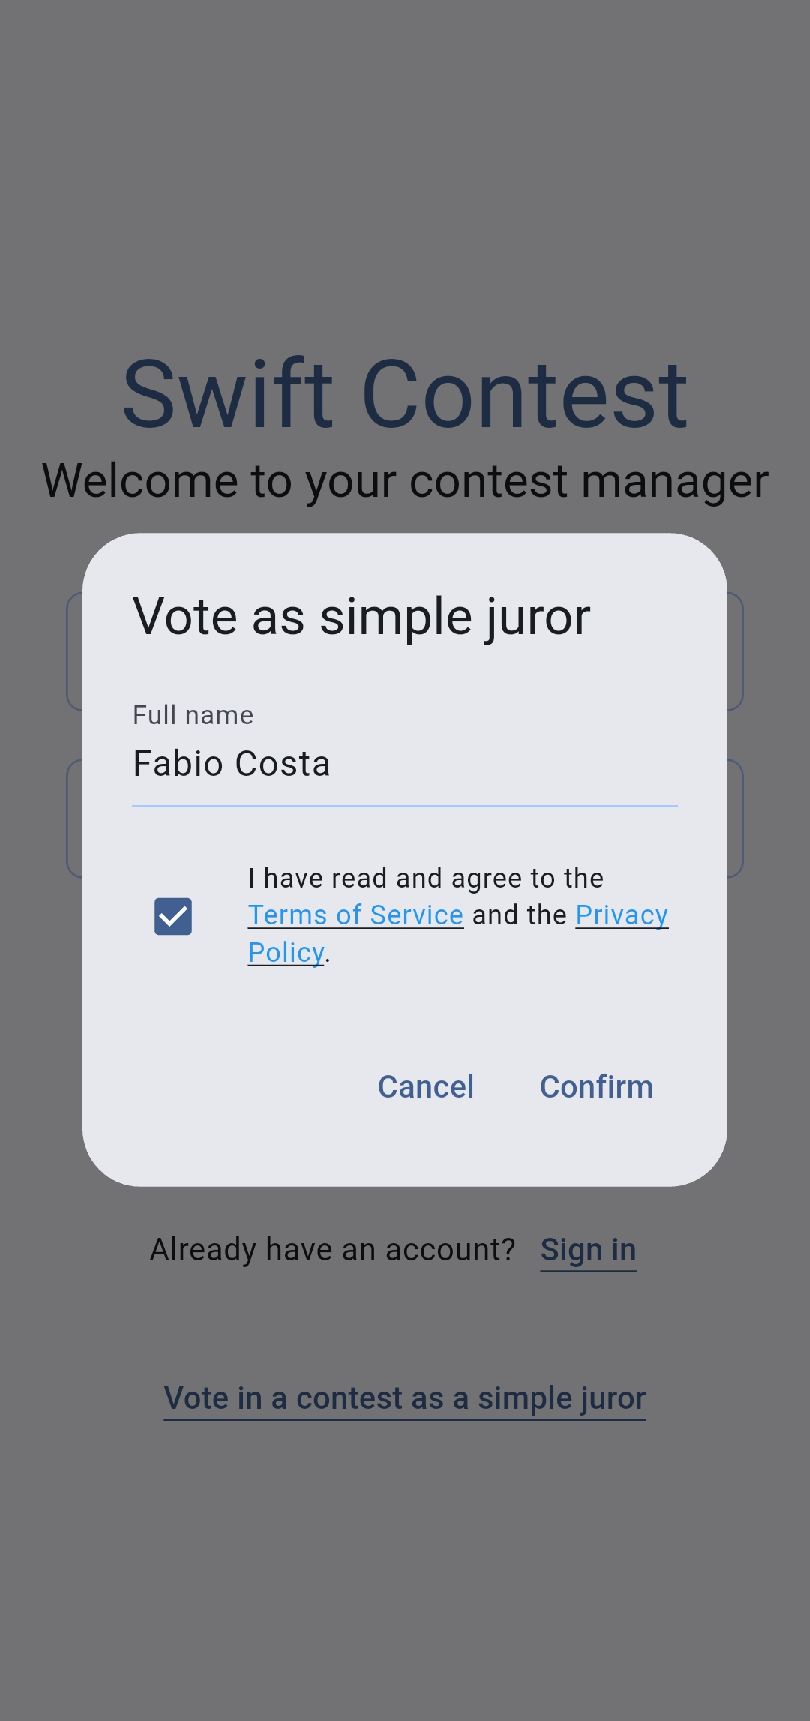
\includegraphics[width=\linewidth]{capitoli/figure/simple-juror/sign-up-form}
        \subcaption{Inserimento nome e cognome}
        \label{fig:simple_juror_name}
    \end{minipage}\hfill
    \begin{minipage}[t]{0.30\textwidth}
        \centering
        
\includegraphics[width=\linewidth]{capitoli/figure/simple-juror/home}
        \subcaption{Home ospite}
        \label{fig:simple_juror_home}
    \end{minipage}
    \caption{I tre passaggi per l'accesso di un giurato semplice (ospite) alla piattaforma.}
    \label{fig:simple_juror_flow}
\end{figure}